\documentclass[tikz,border=2pt]{standalone}
\usepackage{amsmath}
\usetikzlibrary{arrows.meta}
\begin{document}
% QSort([5,2,8,2,9,1]) with pivots 5, then 2 and 8: L=[2,2,1], M=[5], R=[8,9]; then [1],[2,2],[] and
% [],[8],[9]; the leaves read left to right give the sorted list [1,2,2,5,8,9].
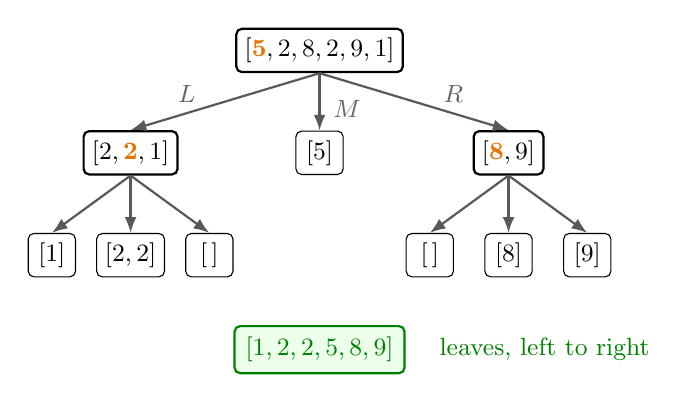
\begin{tikzpicture}[font=\small, >={Latex[length=2mm]},
  call/.style={draw, thick, rounded corners=2pt, inner sep=3pt, minimum height=0.55cm},
  leaf/.style={draw, thin, rounded corners=2pt, inner sep=3pt, minimum height=0.55cm, minimum width=0.6cm}]
  \newcommand{\pv}[1]{\textcolor{orange!90!black}{\boldsymbol{#1}}}
  \node[call] (r) at (0,0) {$[\pv{5},2,8,2,9,1]$};
  \node[call] (l) at (-2.4,-1.3) {$[2,\pv{2},1]$};
  \node[leaf] (m) at (0,-1.3) {$[5]$};
  \node[call] (rr) at (2.4,-1.3) {$[\pv{8},9]$};
  \node[leaf] (ll) at (-3.4,-2.6) {$[1]$};
  \node[leaf] (lm) at (-2.4,-2.6) {$[2,2]$};
  \node[leaf] (lr) at (-1.4,-2.6) {$[\,]$};
  \node[leaf] (rl) at (1.4,-2.6) {$[\,]$};
  \node[leaf] (rm) at (2.4,-2.6) {$[8]$};
  \node[leaf] (rrr) at (3.4,-2.6) {$[9]$};
  \foreach \a/\b in {r/l,r/m,r/rr,l/ll,l/lm,l/lr,rr/rl,rr/rm,rr/rrr}
    \draw[->, thick, gray!70!black] (\a.south) -- (\b.north);
  \node[gray!80!black, anchor=east] at (-1.45,-0.55) {$L$};
  \node[gray!80!black, anchor=west] at (0.05,-0.75) {$M$};
  \node[gray!80!black, anchor=west] at (1.45,-0.55) {$R$};
  \node[green!50!black, draw=green!50!black, thick, fill=green!8, rounded corners=2pt, inner sep=4pt]
    at (0,-3.8) {$[1,2,2,5,8,9]$};
  \node[green!50!black, anchor=west] at (1.4,-3.8) {leaves, left to right};
\end{tikzpicture}
\end{document}
